\documentclass{article}

\usepackage{color}
\usepackage{graphicx}
\usepackage{tabularx}


\usepackage{geometry,wrapfig,lipsum}
 \geometry{
 top=20mm,
 bottom=20mm,
 }


\title{Document pour l'adapation des interfaces}
\author{Justal Kevin}
\date{28/09/2015}
\renewcommand{\contentsname}{Table des mati\`eres} 
 
\newcommand\invisiblesection[1]{%
  \refstepcounter{section}%
  \addcontentsline{toc}{section}{\protect\numberline{\thesection}#1}%
  \sectionmark{#1}} 
 
\begin{document}

\begin{center}
\textbf{\Huge{Bootstrap contre Polymer}}
\line(1,0){300}\\
DOSSIER D'ANALYSE DES DIFFERENCES\\
\vspace{3cm}
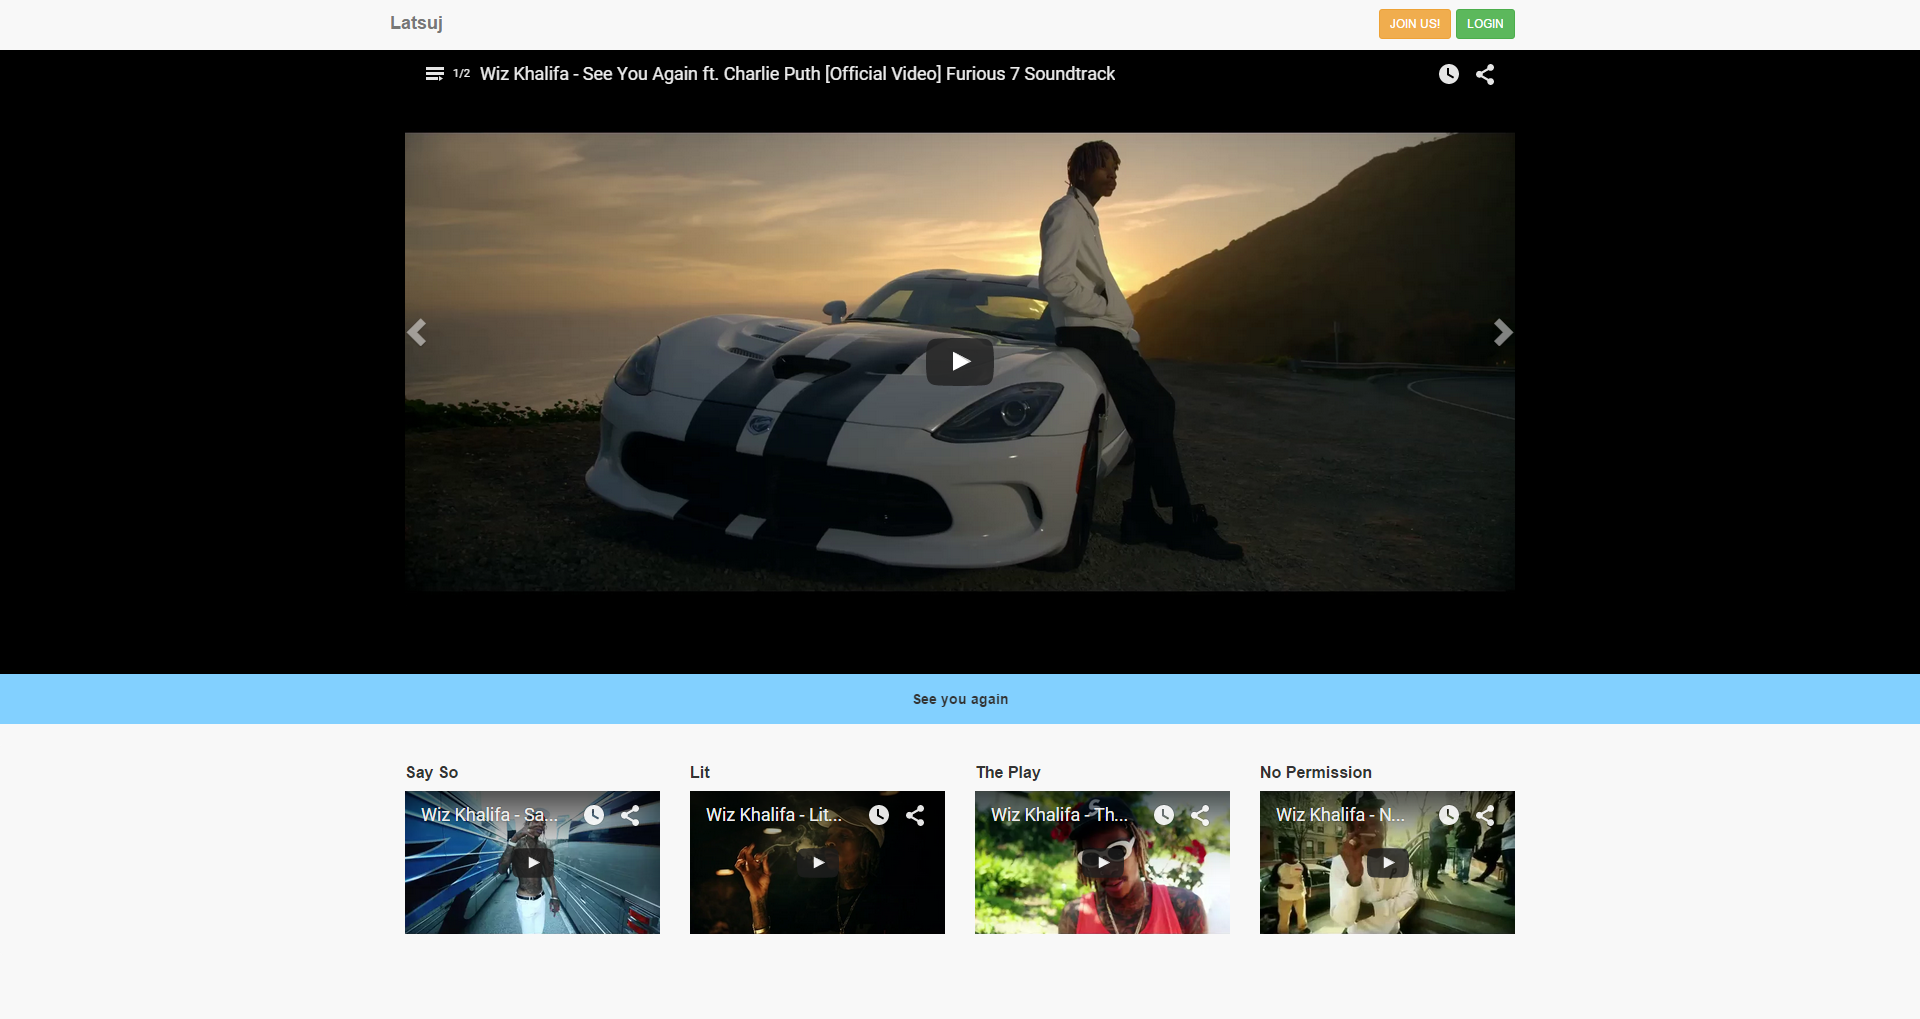
\includegraphics[width=1.0\textwidth]{pc}\\
\vspace{3cm}
\textbf{\Large{JUSTAL KEVIN}}\\
2015\\
\vspace{2cm}
\textbf{Justal Kevin - \color{blue}{\underline{justal@polytech.unice.fr}} \color{black}{- SI5 - IHM}}\\
\vspace{4cm}
\textbf{Enseignant :}\\
\textbf{Anne Marie Dery - \color{blue}{\underline{dery@polytech.unice.fr}}}
\end{center}

\newpage
\newpage
\tableofcontents

\newpage

\section{Comment avez vous r\'ealis\'e l'exemple ?}

Pour r\'ealiser mon exemple, je me suis dans un premier temps int\'eress\'e \`a la d\'efinition m\^eme d'un site web adaptatif. Le principe du RWD (\textit{responsive web design}) ou site web adaptatif dans la langue de moli\'ere consiste \`a s'appuyer sur l'usage des \textit{Media queries}, de grilles de positionnement ou encore d'images flexibles pour rendre un site adaptable \`a son support.\\
Pour d\'evelopper, je suis parti de la version ordinateur, puis j'ai remis en forme les \'el\'ements \`a mesure que la largeur de l'\'ecran diminuait voire je les supprimais totalement. Nous verrons un peu plus loin pourquoi j'ai fait ces choix.
\begin{center}
\vspace{0.5cm}
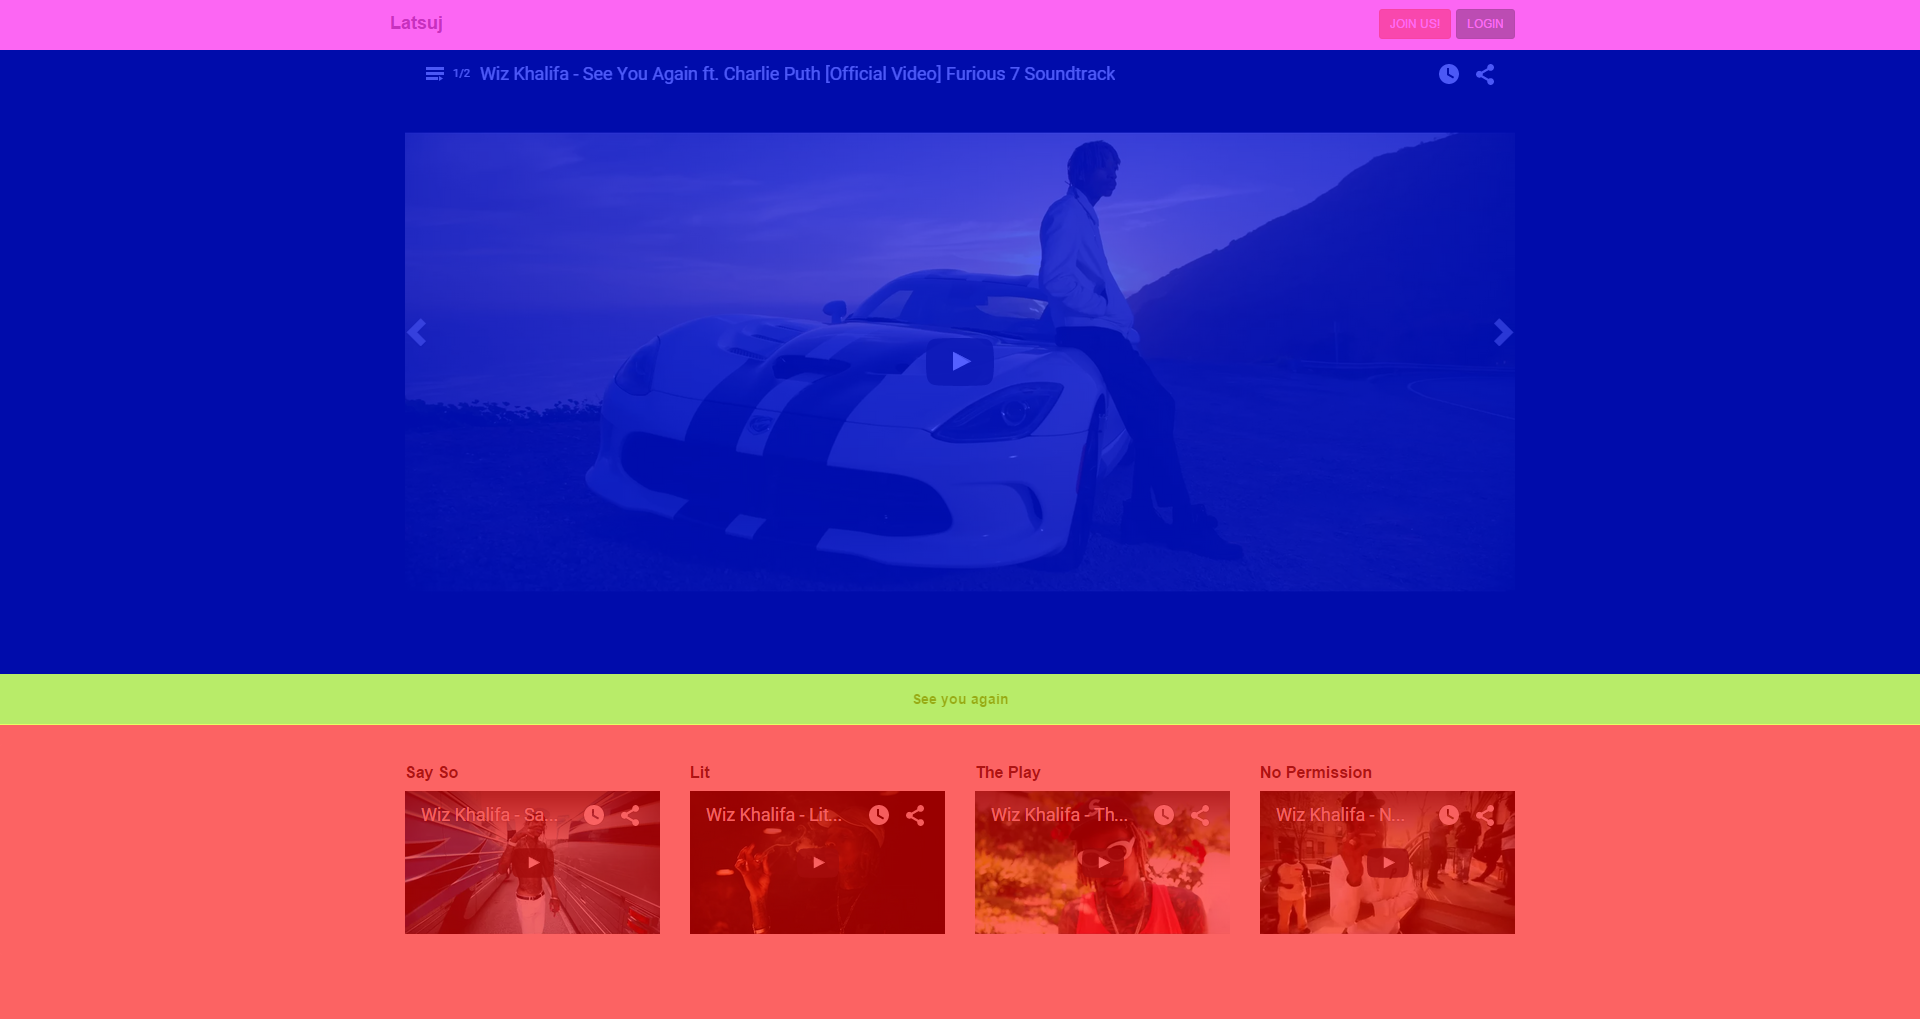
\includegraphics[width=0.8\textwidth]{pc2}
\vspace{0.5cm}
\end{center}

Les deux technologies que j'ai choisie partage la m\^eme structure de base. C'est \`a dire un d\'ecoupage en quatre grands blocs. En rose sur l'image ci-dessus, on trouve la barre de connexion. En bleu, la zone de visionnage des vid\'eo. En Jaune, une zone d'information. Enfin, en rouge, une zone pour afficher les vid\'eos o\`u le chanteur est le m\^eme que la vid\'eo dans la zone bleu.\\
Pour observer pr\'ecis\'ement le principe de RWD, nous allons nous int\'erresser particuli\`erement \`a la zone rouge en bas du site. Cette derni\'ere illustre \`a la perfection tous les aspects que l'on attend d'un site adaptatif. Colorions chaque divisions de cette partie du site d'une couleur unique.
\begin{center}
\vspace{0.5cm}
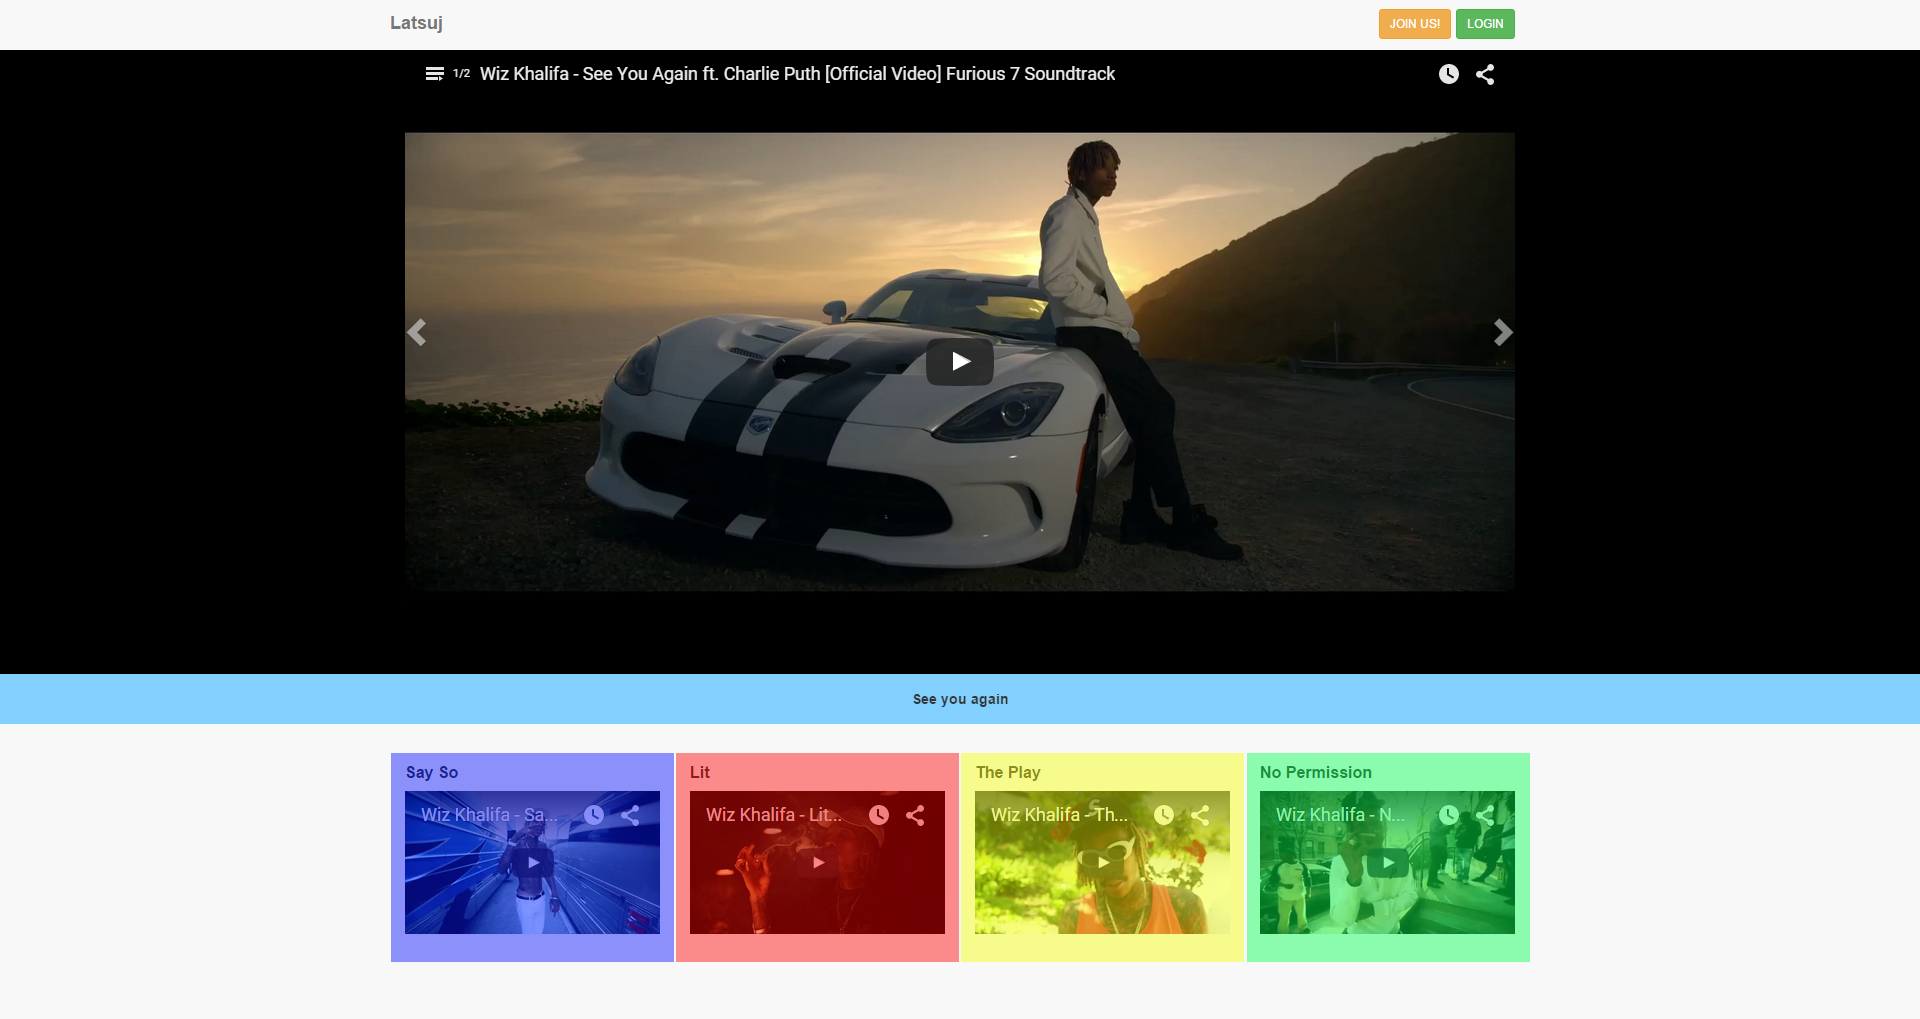
\includegraphics[width=0.8\textwidth]{pc4}
\vspace{0.5cm}
\end{center}
Si nous r\'eduisons la largeur de la fenetre, le contenu s'adaptera. Dans un premier temps, il n'y aura plus que deux blocs par ligne. Puis, si nous continuons de r\'eduire la fen\`etre, il n'y aura plus qu'un seul bloc par ligne et les deux derniers auront \'et\'e cach\'e.
\begin{center}
\vspace{0.5cm}
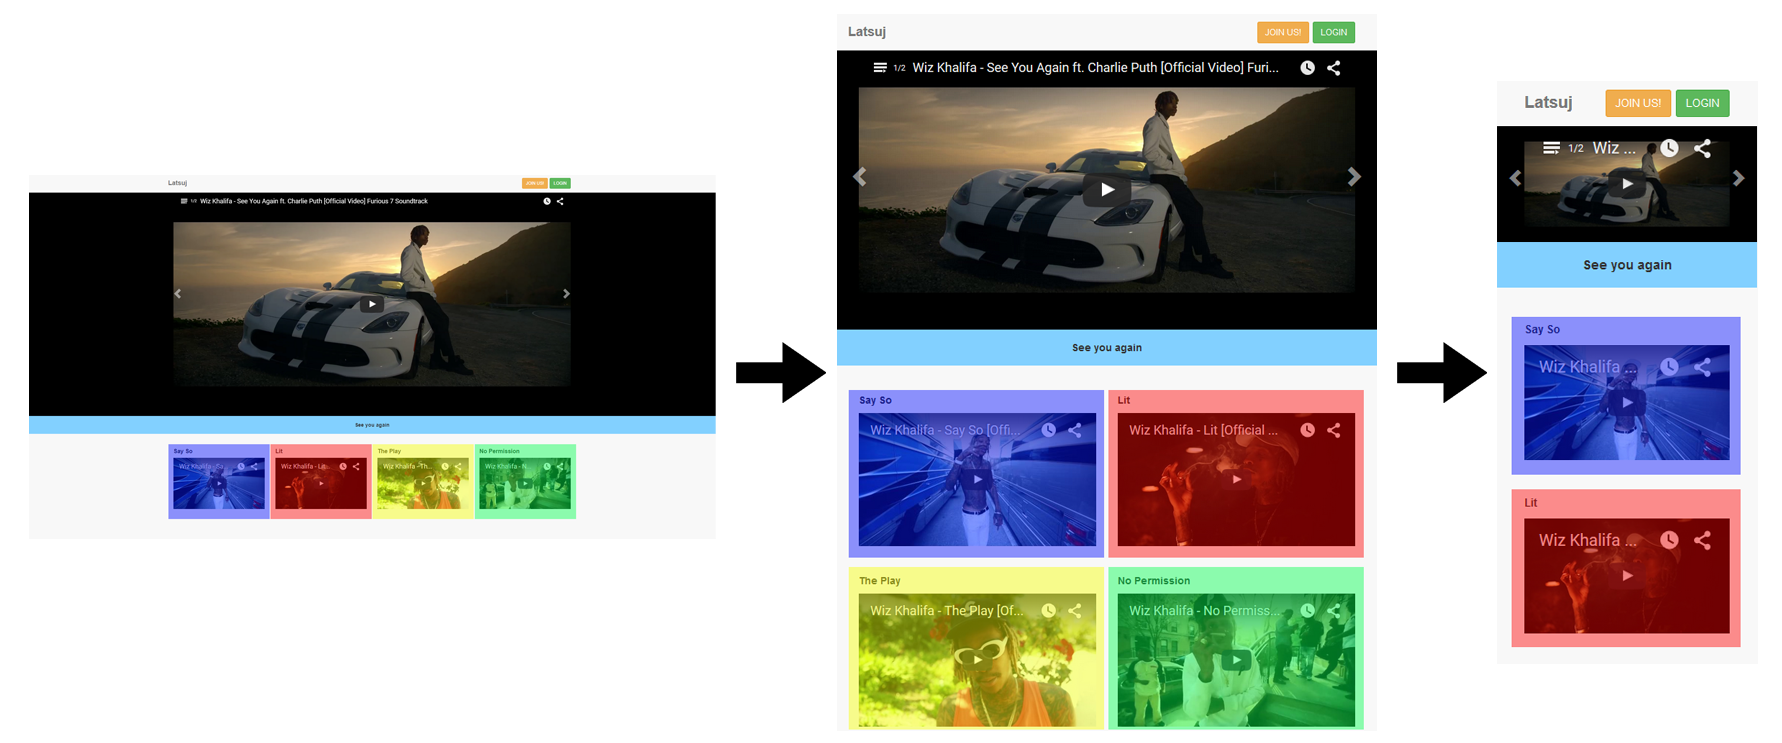
\includegraphics[width=0.8\textwidth]{pc7}
\vspace{0.5cm}\\
\end{center}

Le site s'adapte donc aux dimensions de notre appareil ou fen\`etre.\`A quoi cela peut-il bien servir ? Il serait plus adapté de se demander quels sont probl\`emes que cela r\'esout-il ? Comme on le voit autour de nous, les ordinateurs ne sont plus les seuls \'el\'ements ou gadgets nous entourant, ils existent maintenant une innombrable quantit\'e d'apareil informatique de tous types et de toutes dimensions. Il est important qu'un site internet ne laisse aucun utilisateur sur le bas cot\'e. Comme il est impensable de concevoir une application ou un site internet pour chaque appareil, il faut donc faire un site qui puisse s'adapter suivant les dimensions de l'appareil. 
\vspace{0.5cm}\\
Mais ce n'est pas tout, l'adaptation seul ne permet pas d'\'etablir ce que l'on peut appeler un site web adaptatif. Le cr\'eateur de cette vision, Mr. Ethan Marcotte, a implement\'e un site (\textit{http://alistapart.com/d/responsive-web-design/ex/ex-site-flexible.html}) qui s'adapte \`a la largeur de l'\'ecran. Cependant, il pointe du doigt certains d\'etails. Par exemple, lorsque l'on redimensionne la page, les \'el\'ements vont bel et bien se redimensionner mais les images et le texte \`a tr\`es basse r\'esolution deviendront illisible. Il faut donc que les \'el\'ements se repositionnent dans la page afin que le contenue soit lisible et agr\'eable \`a arpenter pour l'utilisateur. C'est pourquoi dans l'exemple ci-dessus, le nombre de bloc par ligne d\'ecroit au fur et \`a mesure que l'on r\'eduit la fen\^etre.
\vspace{0.5cm}\\

Le site est aussi \textit{responsible typesetting}. La taille en pixel du texte varie suivant la taille de la fen\^etre. Pour l'utilisateur, il est sans aucun doute plus agr\'eable de pouvoir lire les paroles d'une chanson phrase par phrase. Or, si la taille du texte restait la m\^eme pour toutes dimensions de fen\`etre, soit le texte serait illisible \`a une grande r\'esolution, soit le site serait incommode \`a basse r\'esolution. Pour r\'esoudre ce probl\`eme, une proportions a \'et\'e sp\'ecifier pour l'ensemble des textes suivant la largeur de la fen\`etre ou de l'appareil. Sur le site, on retrouve cette particularit\'e sur plusieurs titres et sur les paroles comme nous pouvons le constater ci-dessous. \`A gauche, on retrouve les paroles des chansons sur t\'el\'ephone portable tandis que \`a droite, on retrouve les m\^emes paroles \'ecrite avec une plus grande police sur tablette.
\begin{center}
\vspace{0.5cm}
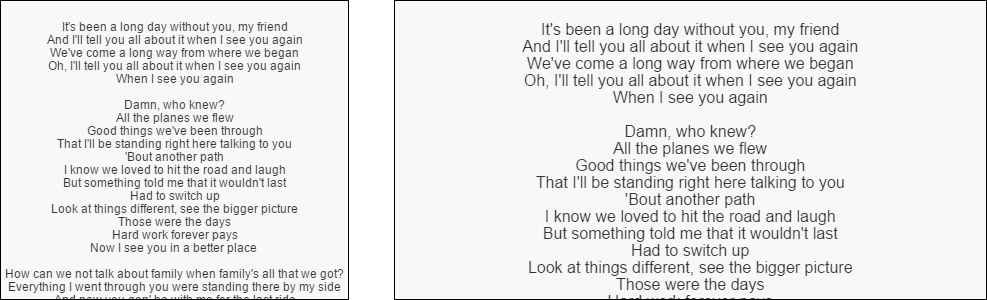
\includegraphics[width=0.8\textwidth]{textes}
\vspace{0.5cm}\\
\end{center}

\newpage

\hspace*{0.6cm}Pourquoi ais-je supprim\'e les deux derniers blocs sur la navigation \`a basse r\'esolution ? Ce n'est pas une d\'ecision anodine. En supprimant ces deux blocs, j'am\'eliore l'exp\'erience de l'utilisateur sur deux aspects.\\
\begin{wrapfigure}{r}{3cm}
\vspace{-13pt}
\centering
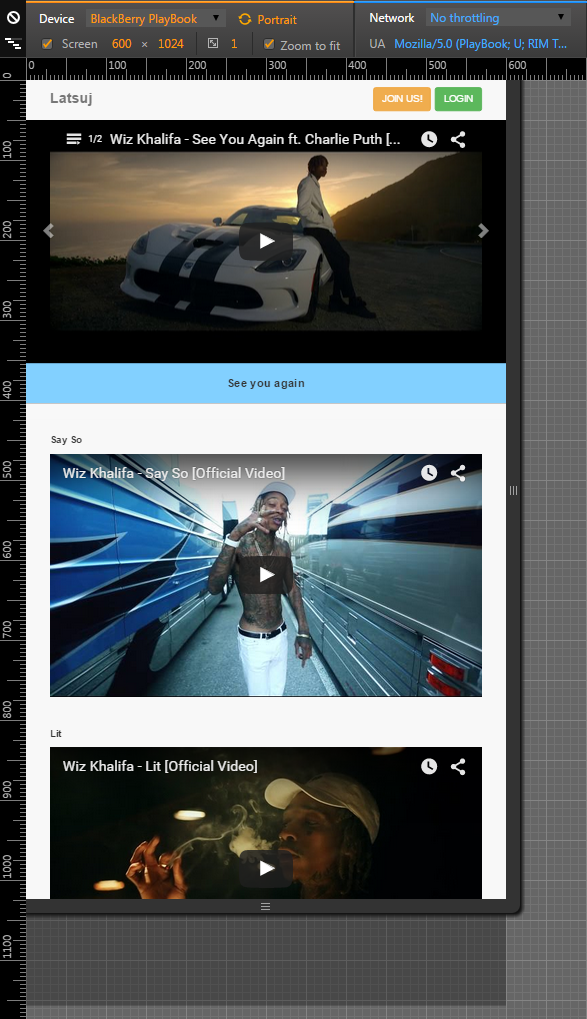
\includegraphics[width=3cm]{blackberry}
\caption{\textit{Affichage du site sous BlackBerry (via Google Chrome).}}
\end{wrapfigure} 
{\hspace*{0.6cm}L'un est purement li\'e \`a la technologie, il est rare d'avoir un t\'el\'ephone branch\'e en Ethernet. Ceci implique que le d\'ebit moyen d'un utilisateur sur t\'el\'ephone est souvent inf\'erieur \`a celui d'un utilisateur sur ordinateur. J'\'evite ainsi \`a l'utilisateur sur t\'el\'ephone de charger trop d'informations qui n'appartiennent pas au contenue principal de la page. Ce ne sont que des publicit\'es pour les autres musiques du m\^eme chanteur. Deuxi\`emement, et c'est sans doute le point le plus important, suivant \textbf{la loi de Fitt}, que je sois sur t\'el\'ephone ou ordinateur l'indice de difficult\'e doit rest\'e le m\^eme. La loi calcul donne un indice de difficult\'e par rapport au temps requis pour aller rapidement d'une position de d\'epart \`a une zone finale de destination. L'utilisateur doit arriver avec la m\^eme rapidit\'e et la m\^eme facilit\'e aux diff\'erentes parties du site. Si l'on regarde l'image sur la droite qui repr\'esente le site sur un t\'el\'ephone BlackBerry, on remarque que le temps pour parvenir \`a la derni\`ere vid\'eo en rapport avec le chanteur est aussi rapide sur le t\'el\'ephone que sur ordinateur. Certes ce n'est pas la m\^eme, mais cela reste la derni\`ere vid\'eo. Si j'avais juste r\'earrang\'e les choses, il aurait d'abord fallu descendre pour arriver \`a la derni\`ere vid\'eo. Cela ne para\^it pas beaucoup plus compliqu\'e mais sans cela, le site se retrouverait complexifi\'e d'apr\`es la loi de Fitts.}\\

\section{Comment teste-t-on les capacit\'es d'adaptations ?}

\hspace*{0.6cm}Pour tester l'affichage et l'adapatation de nos \'el\'ements \`a la fen\^etre, il existe plusieurs voies envisageables. J'ai utilis\'e plusieurs d'entre elle pour effectuer mes tests. La premi\`ere m\'ethode a \'et\'e de modifier la taille de la fen\^etre sous windows.\\
\begin{wrapfigure}[12]{l}{5.5cm}
\vspace{-12pt}
\centering
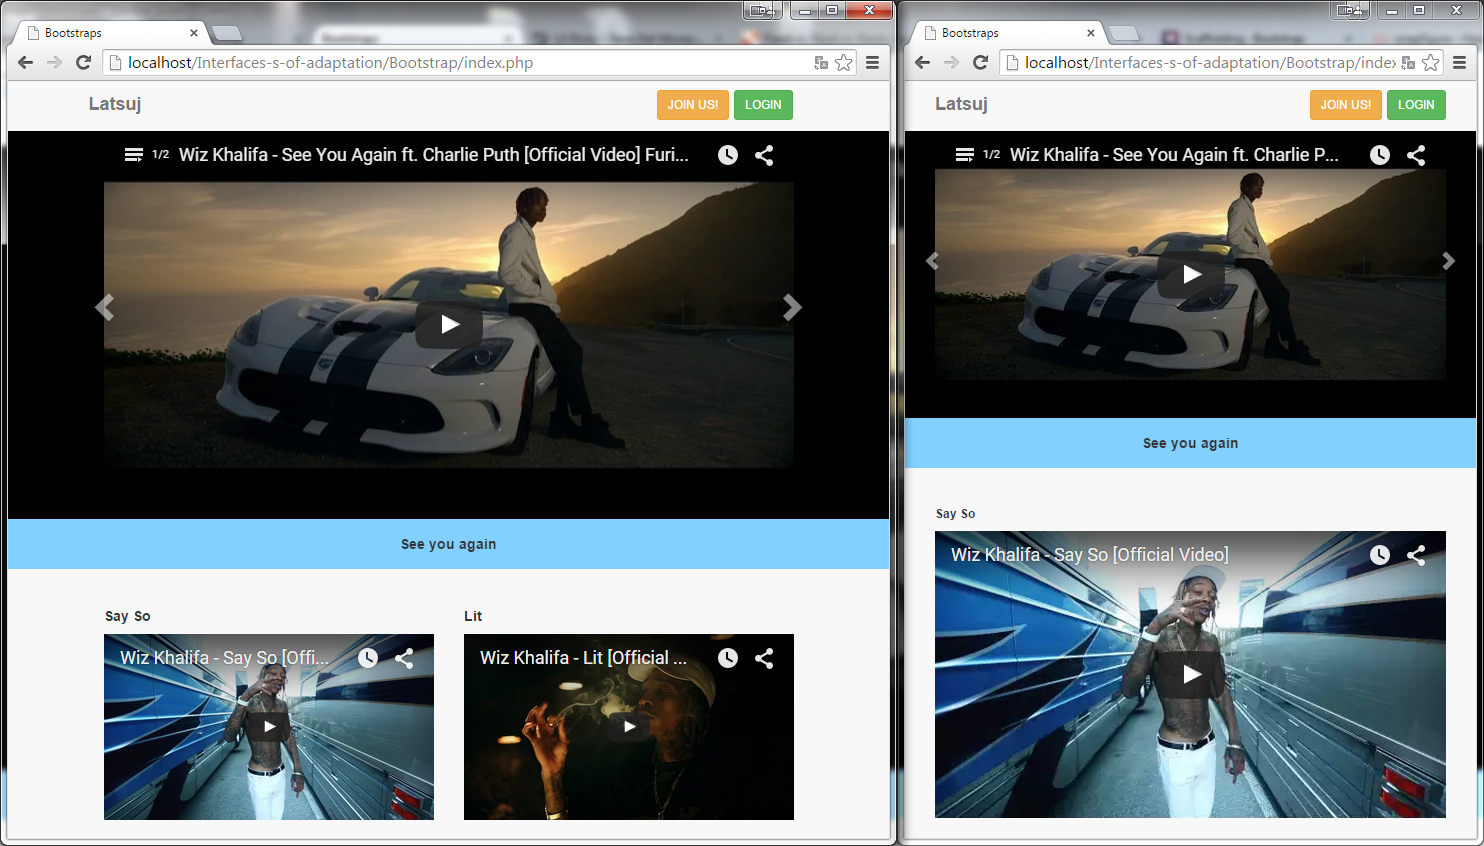
\includegraphics[width=5.5cm]{double}
\caption{\textit{Adaptation du site \`a la largeur de la page.}}
\end{wrapfigure} 
\lipsum[1]

\par

\newpage

\section{Boostraps}


\section{Documentations, Outils, liens utiles} 

\textbf{Wikip\'edia}\\
Le site d'o\'u j'ai d\'emarr\'e mes recherches, il contient une bonne d\'efinition des sites RWD.\\
\textit{https://fr.wikipedia.org/wiki/Site\_web\_adaptatif}
\vspace{0.5cm}\\
\textbf{What is a responsible web design ?}\\
Les liens suivant sont les articles ou vid\'eos que j'ai analys\'e pour \'ecrire ce rapport.\\
\textit{https://www.youtube.com/watch?t=133\&v=iSY38POjLYc}
\vspace{0.5cm}\\
\textbf{Ethan Marcotte}\\
Le site du createur du RWD qui montre la diff\'erence entre un site adpatable et un site responsive.\\
\textit{http://alistapart.com/d/responsive-web-design/ex/ex-site-flexible.html}\\
\textit{http://alistapart.com/d/responsive-web-design/ex/ex-site-linearize.html}
\vspace{0.5cm}\\
\textbf{Responsible typesetting}\\
Un article qui traite du responsible typesetting.\\
\textit{http://blog.line0.eu/responsible-typesetting/}
\vspace{0.5cm}\\
\textbf{Fitt's law}\\
La description de la loi de Fitt\\
\textit{https://en.wikipedia.org/wiki/Fitts's\_law}\\
\textit{http://webdesign.tutsplus.com/articles/applying-fitts-law-to-mobile-interface-design--webdesign-6919}



\section{Difficult\'es rencontr\'es}
\hspace*{0.6cm}Le premier probl\`eme rencontr\'e fut lorsque que j'essaya de coder une balise div de telle mani\`ere que celle-ci remplisse enti\`erement l'espace de l'application. Cette chose extr\`emement simple n'est pourtant pas impl\'ement\'e dans Bootstrap 3.0 et les versions sup\'erieur alors que cela se trouvait dans les versions ant\'erieur avec la class span. Apr\'es de longue recherches, il apparait donc impossible en pur Bootstrap de remplir un div \`a cent pour cent de la balise parent.De ce fait, j'ai du modifi\'e le CSS pour r\'ealiser le remplissage de la page. Pourquoi un tel choix des d\'eveloppeur de bootstrap ?

margin-bottom : Seriously ?

Compatibilite : WTF polymer !

min-height ? WTF do not work !OK parce que tous ces putain d'elements sont en inline et non en block...Ok l'erreur

Suivre un ordre pour appeler les modules au depart, les enfant en premier.

encapsulation des elements ? content :X Merci la doc....pourrie.

Le carousel une horreur sur Polymer....

\section{Simple trouvaille d'optimisation}
En farfouillant sur les documentations de Bootstrap, je suis tomb\'e sur une optimisation qui a retenu mon attention. Une chose simple et pourtant efficace que je ne faisait pas moi non plus. Les developpeurs de Bootstrap mettent toujours les scripts javascript en fin de page afin d'accelerer le chargement de la page. Cela peut paraitre stupide comme remarque mais je tiens \`a m'en souvenir, j'en fait donc par dans mon document.

Petite astuce, enlever les ; sur le dernier elements de css pour gagner un caractere de lecture.

\end{document}
